\documentclass{standalone}
\usepackage{tikz}

\newcommand{\mue}{0}
\newcommand{\sta}{1}
\newcommand{\lowX}{-3}
\newcommand{\lowY}{-0.05}
\newcommand{\hiX}{3}
\newcommand{\hiY}{0.6}

\begin{document}
    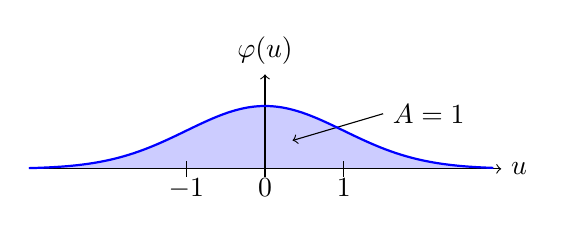
\begin{tikzpicture}[yscale=2]
           
        % Draw and shade the area under the bell curve from x=1 to x=2
        \begin{scope}
            \fill[blue!20] 
            (\lowX,0) -- plot[domain=\lowX:\hiX,smooth] (\x,{1/(\sta*sqrt(2*pi))*exp(-1/2*((\x-\mue)/\sta)^2)}) -- (\hiX,0) -- cycle;
        \end{scope}
    
        \draw[<-] (0.35,0.18) -- (1.5,0.35) node[right]{$A=1$};
  
        % Draw the x and y axes
        \draw[->] (\lowX,0) -- (\hiX,0) node[right] {$u$};
        \draw[->] (0,\lowY) -- (0,\hiY) node[above] {$\varphi(u)$};

        % Lines from y=0 to curve
        \draw[black] (-1,-0.05) -- (-1,0.05);
        \draw[black] (1,-0.05) -- (1,0.05);
        % \draw[black, dashed, thick] (\mue,0) -- (\mue,0.4);
        % \draw[black] (4,0) -- (4,0.24);

        % Draw the bell curve
        \draw[scale=1.0,domain=\lowX:2.9,smooth,variable=\x,blue,thick,samples=100] 
            plot ({\x},{1/(\sta*sqrt(2*pi))*exp(-1/2*((\x-\mue)/\sta)^2)});
        
    
        % Optionally, add labels
        \node[below] at (0,0) {$0$};
        \node[below] at (-1,0) {$-1$};
        % \node[below] at (\mue,0) {$\mu$};
        \node[below] at (1,0) {$1$};
    \end{tikzpicture}
\end{document}
